\section{Log Extension} \label{sec:log}
Now we shift our focus towards detecting some types of log misbehavior, namely,
omission attacks.  The design idea is an
extension of our base design.  A prerequisite is that the CT log landscape
is modified to support \emph{SCT cross-logging}.  Cross-logging refers to the
idea of logging signed statements in other logs to intertwine
them, thus making it more difficult to get away with
misbehavior.  We use the general idea and apply it to SCTs.  This means that
CTRs can log SFOs rather than certificate chains, making it possible to detect
MMD violations.

\subsection{Design Sketch}
Figure~\ref{fig:ext-log} provides an overview of the extended design.  Tor
Browser submits presented SFOs probabilistically to CTRs that are selected
at random, and CTRs mix the submitted SFOs before any auditing takes place.
Here, auditing refers to the submission of full SFOs rather than the underlying
certificate chains.  There are four changes when compared to the design in
Section~\ref{sec:base}:
(i) MMDs of CT logs that Tor Browser recognizes must be added to the Tor
consensus,
(ii) how a CTR mixes the received SFOs,
(iii) what is submitted to the logs, and
(iv) CTRs publish metrics in the extra-info document.

\begin{figure*}
    \centering
    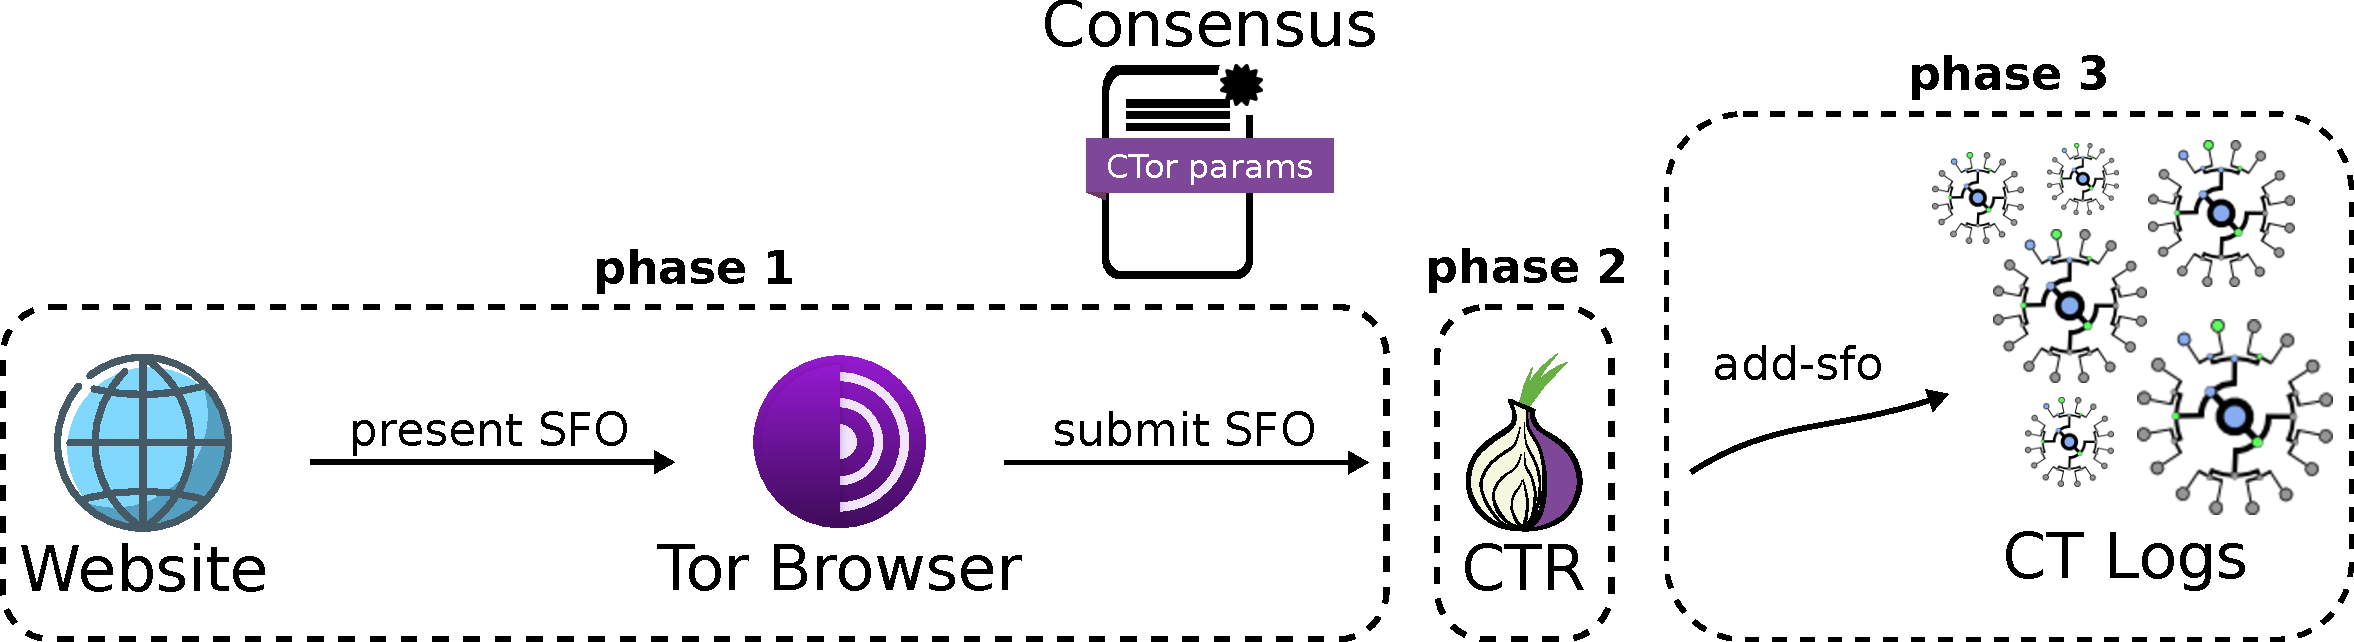
\includegraphics[width=0.85\textwidth]{img/design-log}
	\caption{TODO: Tobias, s/submit-entry/submit-sfo}
    \label{fig:ext-log}
\end{figure*}

Starting backwards with phase~3, CT logs need an endpoint that accepts SCTs in
addition to certificate chains.  We refer to this endpoint as
\texttt{submit-sfo}, and CTRs use it instead of \texttt{add-chain} or
\texttt{submit-entry}.  The submitted SCTs are of particular interest,
considering that they contain timestamps that reveal whether the issuing CT logs
violated their MMD promises by not incorporating a certificate chain on time.
Note that \emph{anyone} can inspect the cross-logged SFOs further, which in
themselves prove misbehavior beyond doubt:
	an SCT is digitally signed by the issuing CT log, and
	it is cryptographically binding with regards to a certificate chain.

To increase the probability of catastrophic impact for the attacker by detecting
omissions, it is paramount that there are no \emph{early signals} that
allow the CT logs in question to reactively merge certificate chains before
any MMD is violated.  Therefore, \texttt{audit\_after} timestamps should be
computed as follows in phase~2 with regards to the SCT and MMD that yields the
largest max-value:

\begin{equation} \label{eq:audit-after}
	\begin{aligned}
		t \gets& \mathsf{random\_delay}(\texttt{ct-delay-dist})\;+ \\
		&\mathsf{max}(
			\mathsf{now}(),
			\textrm{SCT}.\mathsf{timestamp}+\mathsf{MMD}
		).
	\end{aligned}
\end{equation}

Assuming no future-dated SCTs which follow from the mandated TLS client behavior
in RFC~6962~\cite{ct}, the \texttt{audit\_after} timestamp in
Equation~\ref{eq:audit-after} assures that a cross-logged SFO entails proof
of certificate omission.  As discussed next, the possibility of larger
\texttt{audit\_after} timestamps introduces the threat of network-wide flushes.
To facilitate detection, CTRs should publish received and deleted SFO-bytes in
the extra-info document.  This can be compared to existing and similar
extra-info metrics, such as a Tor relay's \texttt{read-history}.

%
% Tor consensus
% - Need MMD
%

%
% Phase 1---Tor browser
% - No changes
%

%
% Phase 2---Storage
% - Updated steps to compute an audit_after timestamp.
%   --> Should we still base on random SCT, or max MMD?
%

%
% Phase 3---Auditing
% - Updated submission endpoint, i.e., submit SFO rather than cert chain
%

%
% Extra-info document
% - Need flushing statistics
%

\subsection{Security Sketch}
%
% MISC notes
% - Network-wide flush, detectable but hard to attribute
% - Requires that the logs extend their APIs to accept SCT cross-logging
%
